\documentclass{article}
\usepackage[utf8]{inputenc}
\usepackage{polski}
\usepackage{geometry}
\usepackage{pdfpages}
\usepackage{pdfpages}
\usepackage{listings}
\usepackage{listingsutf8}
\usepackage{multirow}
\usepackage{siunitx}
\usepackage{multirow}
\usepackage{booktabs}
\usepackage{tabularx}
\usepackage{placeins}
\usepackage{pdflscape}
\usepackage{graphicx}
\usepackage{subfig}
\usepackage{hyperref}
\usepackage{amsmath}
\usepackage{colortbl}
\usepackage[hidelinks]{hyperref}

\geometry{
a4paper,
total={170mm,257mm},
left=20mm,
top=20mm
}
\newcolumntype{Y}{>{\centering\arraybackslash}X}
\renewcommand\thesection{}
\renewcommand\thesubsection{}

\lstset{%
literate=%
 {ą}{{\k{a}}}1
 {ę}{{\k{e}}}1
 {Ą}{{\k{A}}}1
 {Ę}{{\k{E}}}1
 {ś}{{\'{s}}}1
 {Ś}{{\'{S}}}1
 {ź}{{\'{z}}}1
 {Ź}{{\'{Z}}}1
 {ń}{{\'{n}}}1
 {Ń}{{\'{N}}}1
 {ć}{{\'{c}}}1
 {Ć}{{\'{C}}}1
 {ó}{{\'{o}}}1
 {Ó}{{\'{O}}}1
 {ż}{{\.{z}}}1
 {Ż}{{\.{Z}}}1
 {ł}{{\l{}}}1
 {Ł}{{\l{}}}1
}

\title{Metody Obliczeniowe w Nauce i Technice\\ 
Laboratorium VI}
\author{Maciej Trątnowiecki}
\date{AGH, Semestr Letni, 2020}

\begin{document}
    \maketitle
    \section{Zbiór dokumentów testowych}
        Program przygotowany został do indeksowania artykułów z wikipedii. Jako zbiór stron indeksowanych przez wyszukiwarkę przyjąłem wszystkie artykuły linkowane na stronach wymienionych w ustawieniach programu. Program testowałem dla wszystkich artykułów linkowanych na stronie \url{https://en.wikipedia.org/wiki/List_of_Toyota_vehicles}.\\
        
        Otrzymałem w ten sposób zbiór około sześciuset dokumentów w formacie \textit{.html}, oraz wektor termów długości $36857$ elementów. 
        
    \section{Przetwarzanie wstępne zbioru dokumentów}
        Przed uruchomieniem serwera wyszukiwarki przeprowadzane jest wstępne przetwarzanie zdefiniowanych źródeł. Ze względu na dużą złożoność obliczeniową tego zadania, wykorzystywane jest przetwarzanie wielowątkowe, oraz cacheowanie przetworzonych danych. Pliki źródłowe realizujące wstępne przetwarzanie zdefiniowane są wewnątrz modułu \textit{preprocessing}.\\
        \subsection{Przetwarzanie źródeł dokumentów}
        Najpierw, za pomocą prostego \textit{crawlera} znajdującego się w module \textit{gather\_pages} wykonanego w oparciu o \textit{BeautifulSoup} zbierane są wszystkie linki znajdujące się na stronach wymienionych w pliku konfiguracyjnym. Następnie, strony te są kolejno pobierane do folderu \textit{wiki\_pages} na dysku. Na tym etapie lokalnej bazie sqlite3 aplikacja zapisuje tytuł pobranego dokumentu, link do wikipedii z którego został pobrany, oraz ścieżkę do lokalnego pliku na dysku. 
        
        \subsection{Przetwarzanie pojedynczego artykułu}
        Następnie, gdy wszystkie dokumenty zostaną zapisane, z bazy danych ładowany jest zbiór wszystkich dokumentów wymagających wczytania. Dokumenty te są przetwarzane za pomocą modułu \textit{words}. Początkowo, dokument jest tokenizowany za pomocą biblioteki \textit{html2text}. Z pliku wydobywane są wyłącznie wyrazy nie będące częścią linków, ścieżek obrazów, oraz innych elementów definiujących strukturę pliku \textit{html}. Następnie, każde ze słów jest sprowadzane do małych liter, przeprowadzany jest jego \textit{stemming} za pomocą biblioteki \textit{nltk}. Ignorowane są wyrazy pomocnicze, oraz napisane za pomocą liter alfabetu innego niż łaciński. Usuwane są też znaki specjalne, oraz cyfry. \\
        
        Otrzymany w ten sposób dla każdego z artykułów multizbiór wyrazów \textit{cacheowany} jest w bazie danych.
    
        \subsection{Budowa macierzy wektorów \textit{bag of words}}
        Następnie, wyznaczana jest lista termów dla przygotowanego w poprzednich krokach zbioru artykułów. Stanowi on uporządkowaną leksykograficznie listę wyrazów występujących we wszystkich artykułach bez powtórzeń.\\
        
        Na podstawie listy termów wyznaczane są wektory \textit{bag of words} dla wszystkich artykułów. Są one przechowywane jako macierze rzadkie, z wykorzystaniem modułu \textit{scipy.sparse} (macierz \textit{csr\_matrix}). Wektory te nie są zapisywane w bazie danych (choć możliwe by to było choćby z wykorzystaniem pola \textit{BLOB} lub innej metody serializacji macierzy rzadkich). Po uzyskaniu wszystkich wektorów, budowana jest macierz powstała poprzez zebranie ich w porządku leksykograficznym. \\
        
        Otrzymana w ten sposób macierz przemnożona została przez wektor inverse document frequency. Celem tej transformacji jest wyrównanie znaczenia pomiędzy częściej i rzadziej występującymi w tekście słowami podczas wyszukiwania. Następnie macierz aproksymowana jest z wykorzystaniem \textit{low rank approx}, oraz dekompozycji svd. Stopień aproksymacji $k$ wyznaczany jest na podstawie liczby dokumentów. Zależność liniowa stopnia aproksymacji względem liczby artykułów dobrana została eksperymentalnie dla testowanego zbioru opisanego w pierwszym paragrafie tego sprawozdania. 
        
    \section{Wyszukiwanie wprowadzonego hasła}
        Po wprowadzeniu zapytania przez użytkownika, przedstawiane jest ono w postaci wektora \textit{bag of words}. Następnie, liczona jest korelacja wyprowadzonego wektora z wektorami w macierzy odpowiadającymi za kolejne strony. Jako wynik wyszukiwania zwracane jest \textit{n\_pages} artykułów o najwyższej korelacji, gdzie \textit{n\_pages} jest parametrem funkcji odpowiadającej za wyszukanie (domyślnie 10).\\
        
        Korelacja pomiędzy wektorem odpowiadającym zapytaniu, a wektorem odpowiadającym za stronę wyznaczana jest jako iloczyn dwóch powyższych. W celu przyśpieszenia działania, funkcja wyszukująca operuje na macierzy w postaci \textit{numpy ndarray}, w przeciwieństwie do macierzy rzadkiej \textit{csr\_matrix} wykorzystywanej w poprzednich krokach. W razie potrzeby (to jest gdy macierz którą chcemy wykorzystać nie mieści się w klasycznej postaci w pamięci komputera) wykorzystać możemy macierz rzadką, kosztem wydajności. 
        
        \subsection{Interfejs graficzny}
        Aplikacja wyposażona została w prosty interfejs graficzny.
        \begin{figure}[h!]
            \centering
            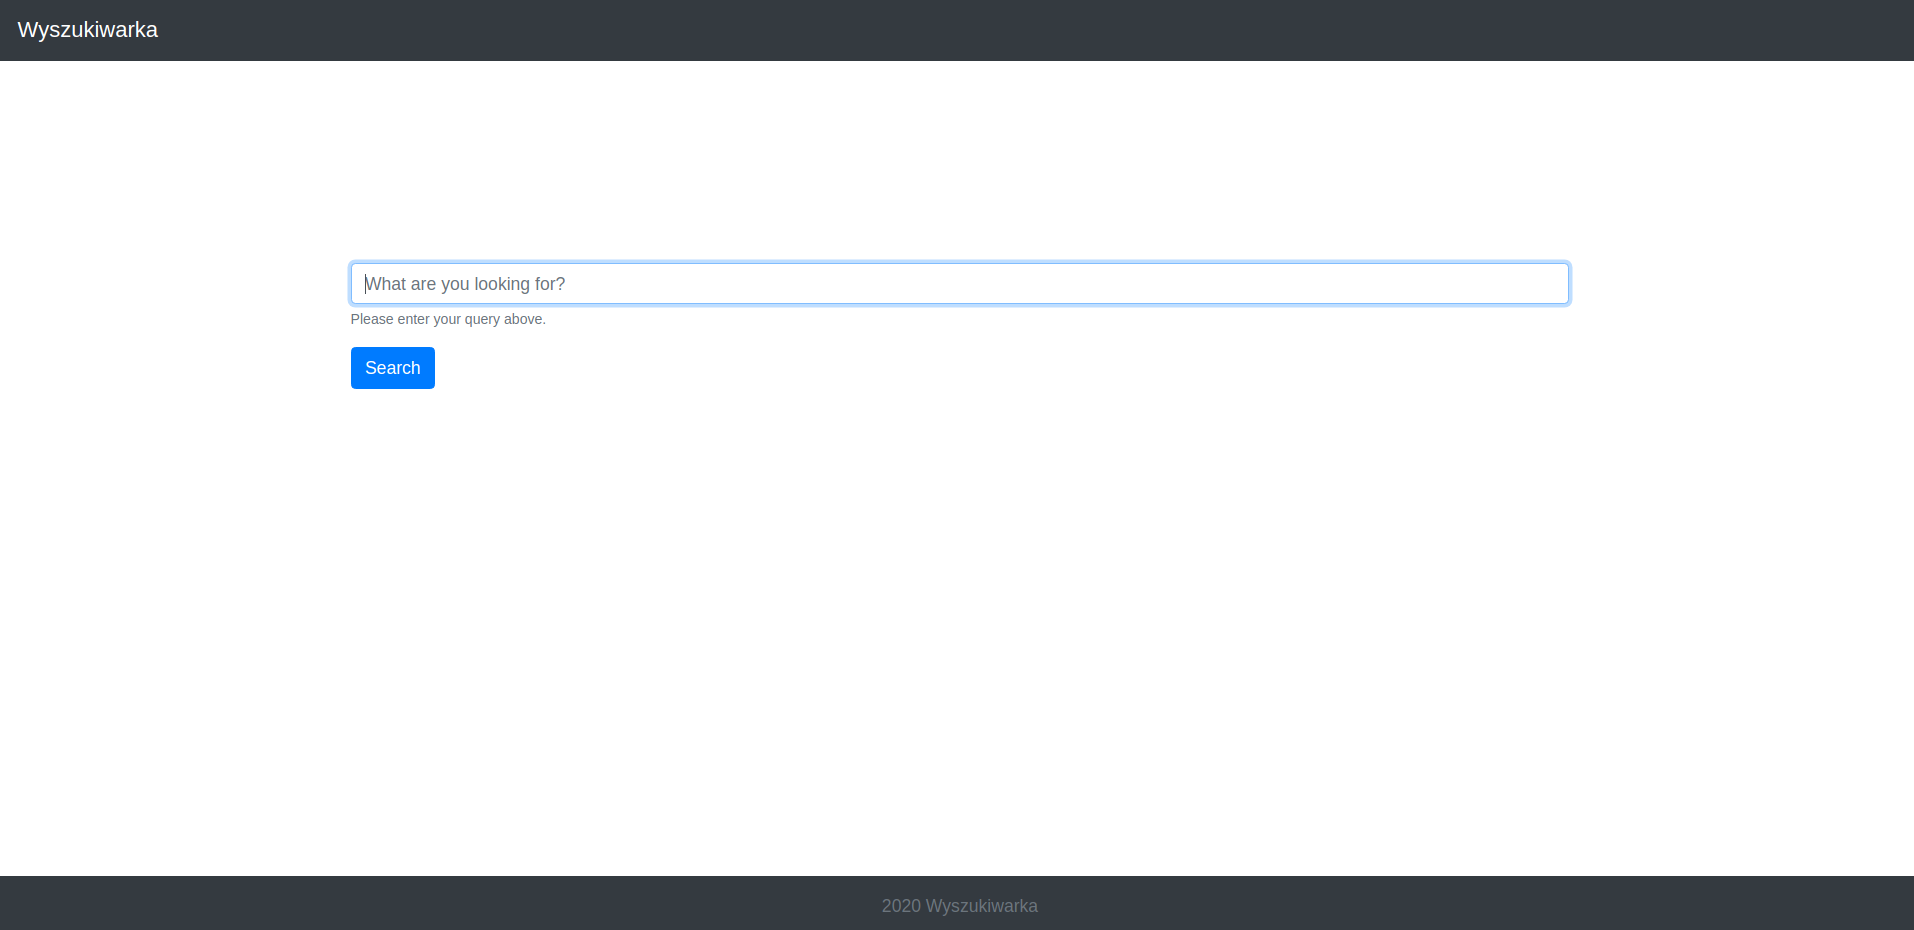
\includegraphics[width=14cm]{lab6/img/front_index.png}
            \caption{Główna strona wyszukiwarki}
        \end{figure}\\
        Został on wykonany w formie aplikacji internetowej opartej o framework \textit{Flask}. \\
        Wyniki zapytania wyświetlane są wraz z odnośnikami do strony z której pochodzą, oraz wyznaczoną korelacją. 
        \begin{figure}[h!]
            \centering
            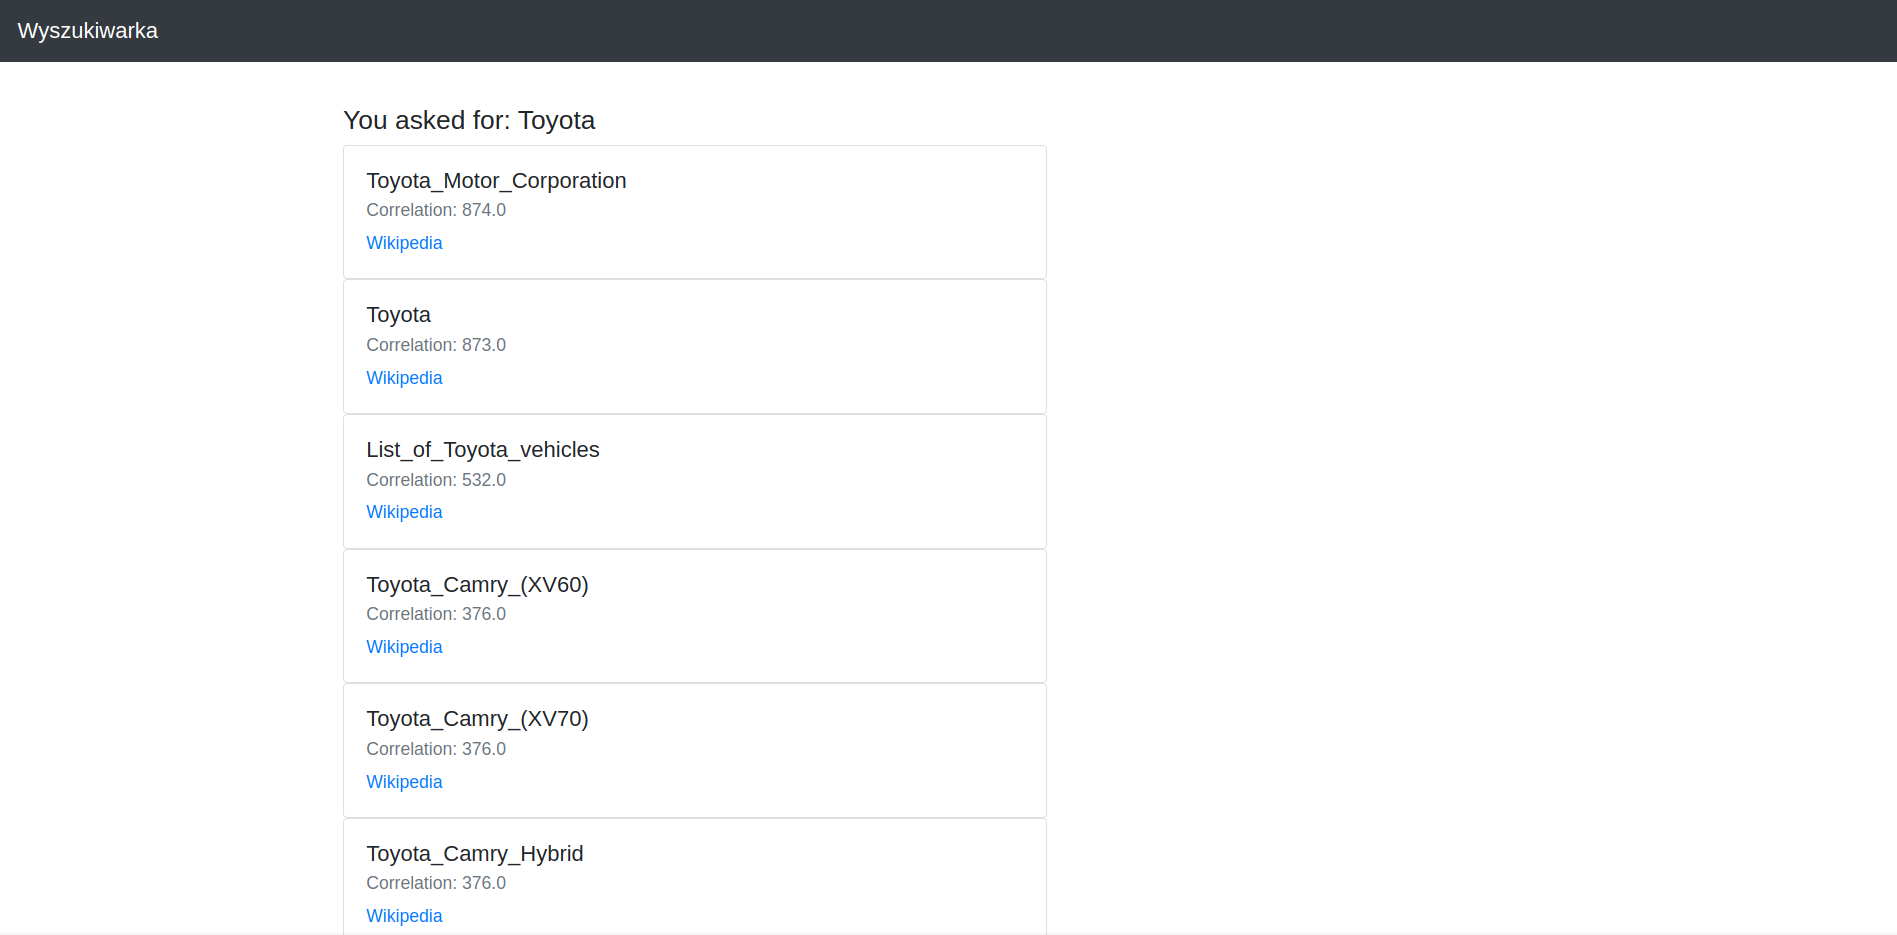
\includegraphics[width=14cm]{lab6/img/front_result1.png}
            \caption{Przykładowe wyniki zapytania}
        \end{figure}\\
        \FloatBarrier

        \subsection{Badanie optymalnego stopnia aproksymacji \textit{low rank}}
        Optymalny stopień aproksymacji dobrany został w sposób empiryczny dla przyjętego w pierwszym paragrafie zbioru testowego dokumentów. Macierz wektorów \textit{bag of words} odpowiadających za kolejne strony aproksymowana była przy pomocy parametru $k$ o wartościach kolejno ${20,40,60,80,100,300}$, oraz ilości dokumentów. Na podstawie tak przeprowadzonych testów ustaliłem w sposób subiektywny, że wartość współczynnika może wynosić około $80$, bez znaczącej utraty dokładności. Odpowiada to około $\frac{13}{100}$ ilości zindeksowanych artykułów. 
        
        \newpage
        \begin{figure}[h!]
            \centering
            \subfloat[$k=20$]{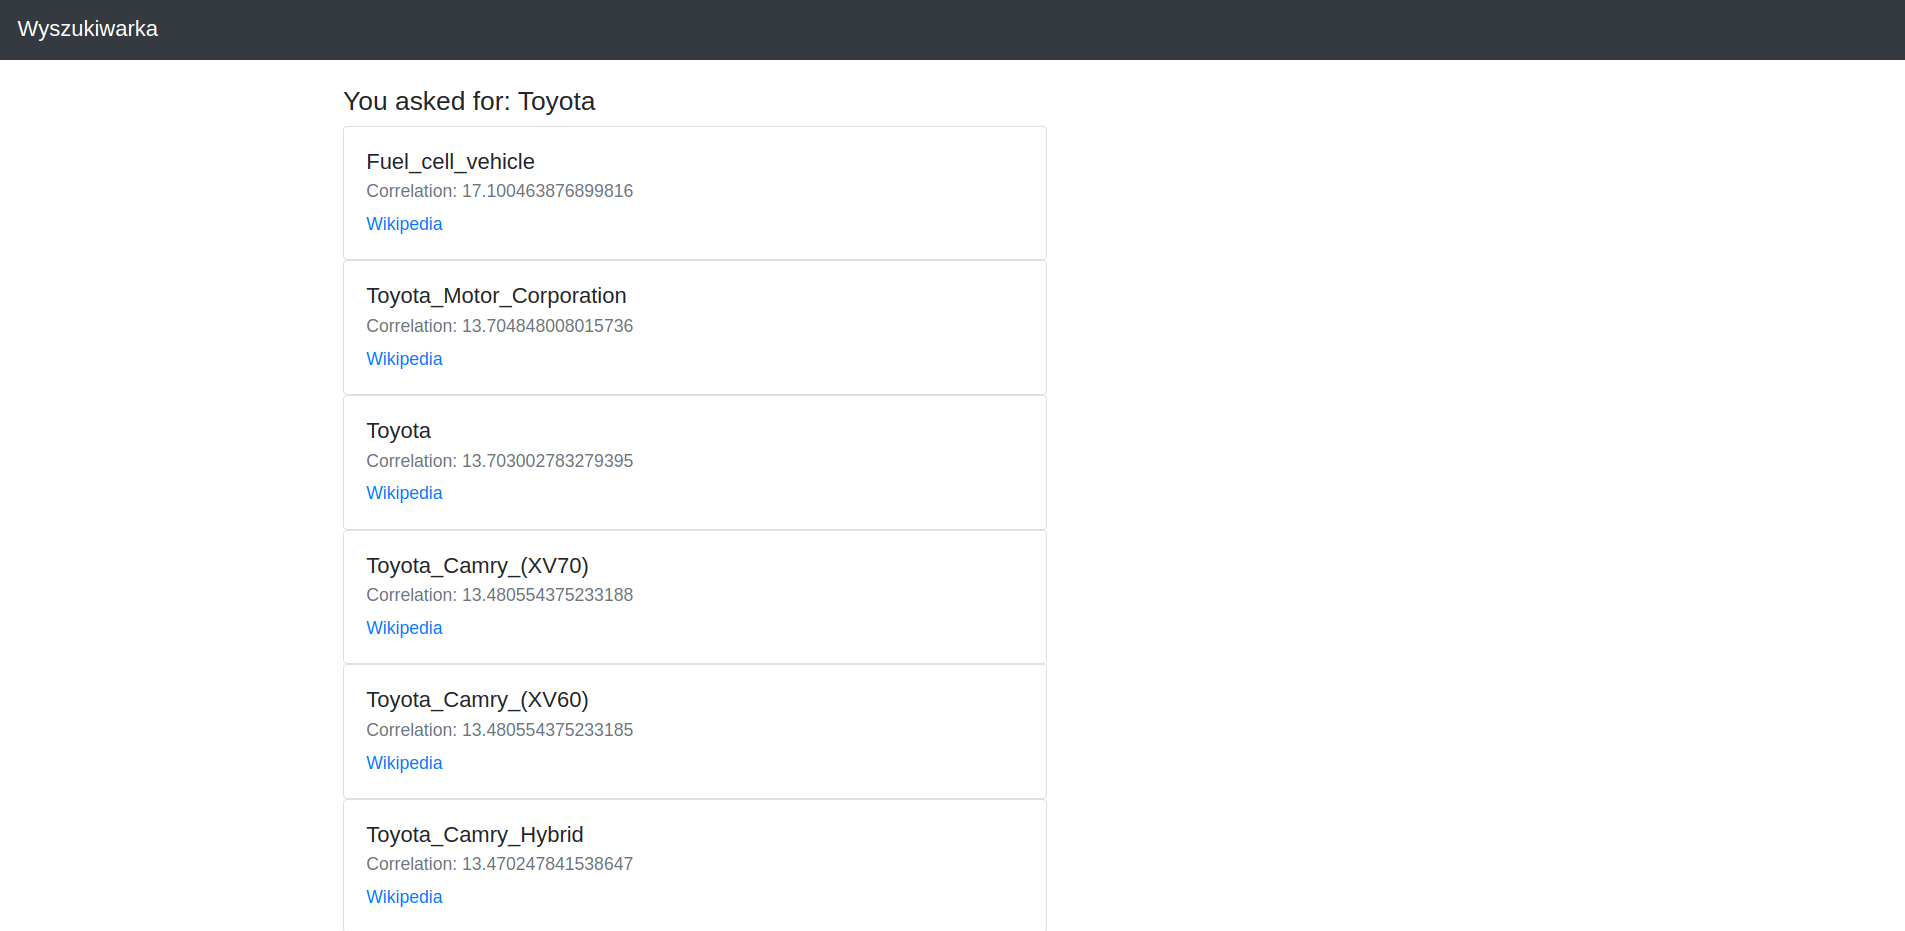
\includegraphics[height=10cm]{lab6/img/front_result1_k20.png}}
            \subfloat[$k=40$]{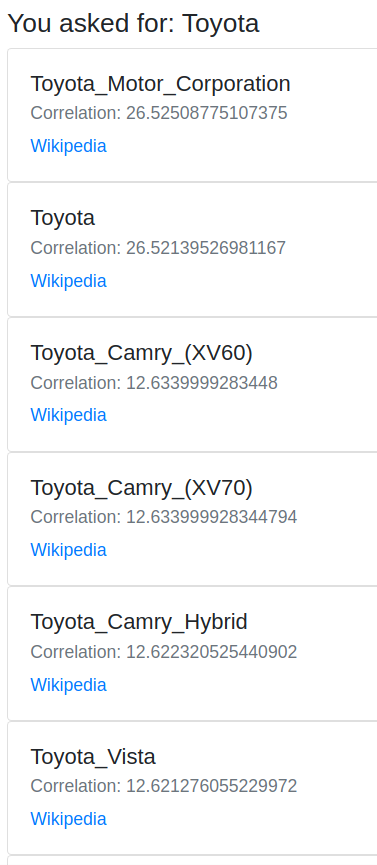
\includegraphics[height=10cm]{lab6/img/front_result1_k40.png}}
            \subfloat[$k=60$]{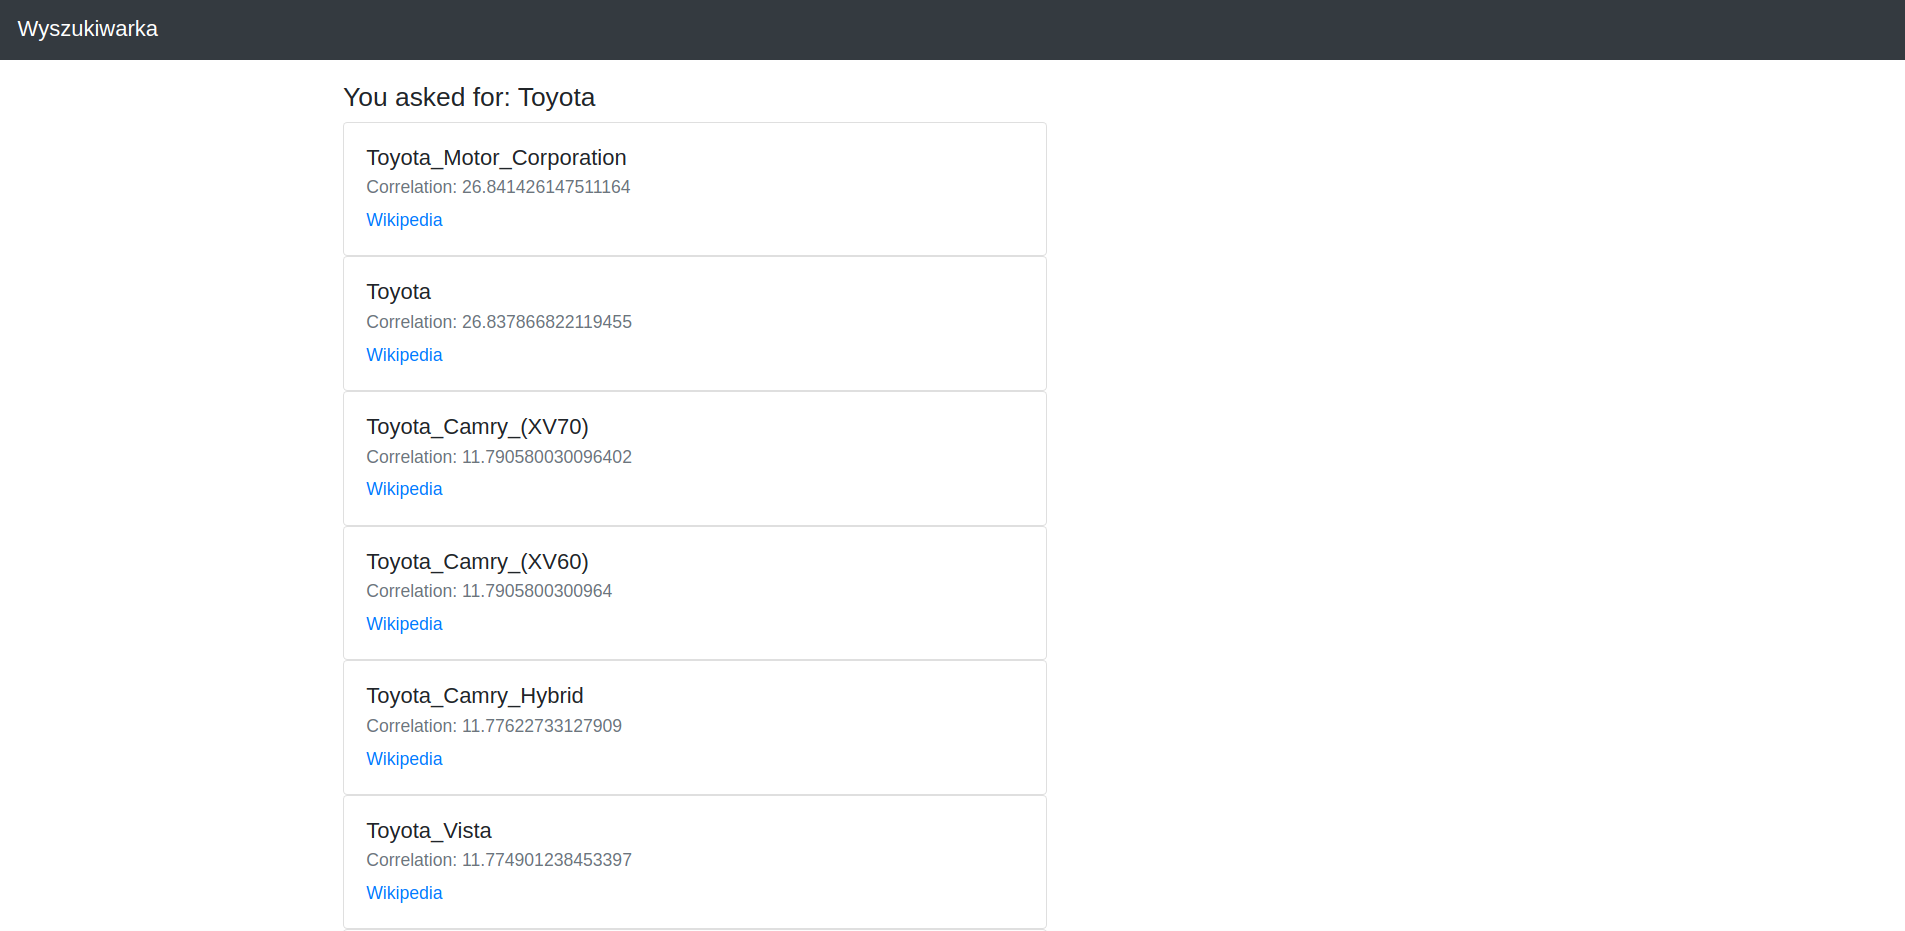
\includegraphics[height=10cm]{lab6/img/front_result1_k60.png}}\\
            \subfloat[$k=80$]{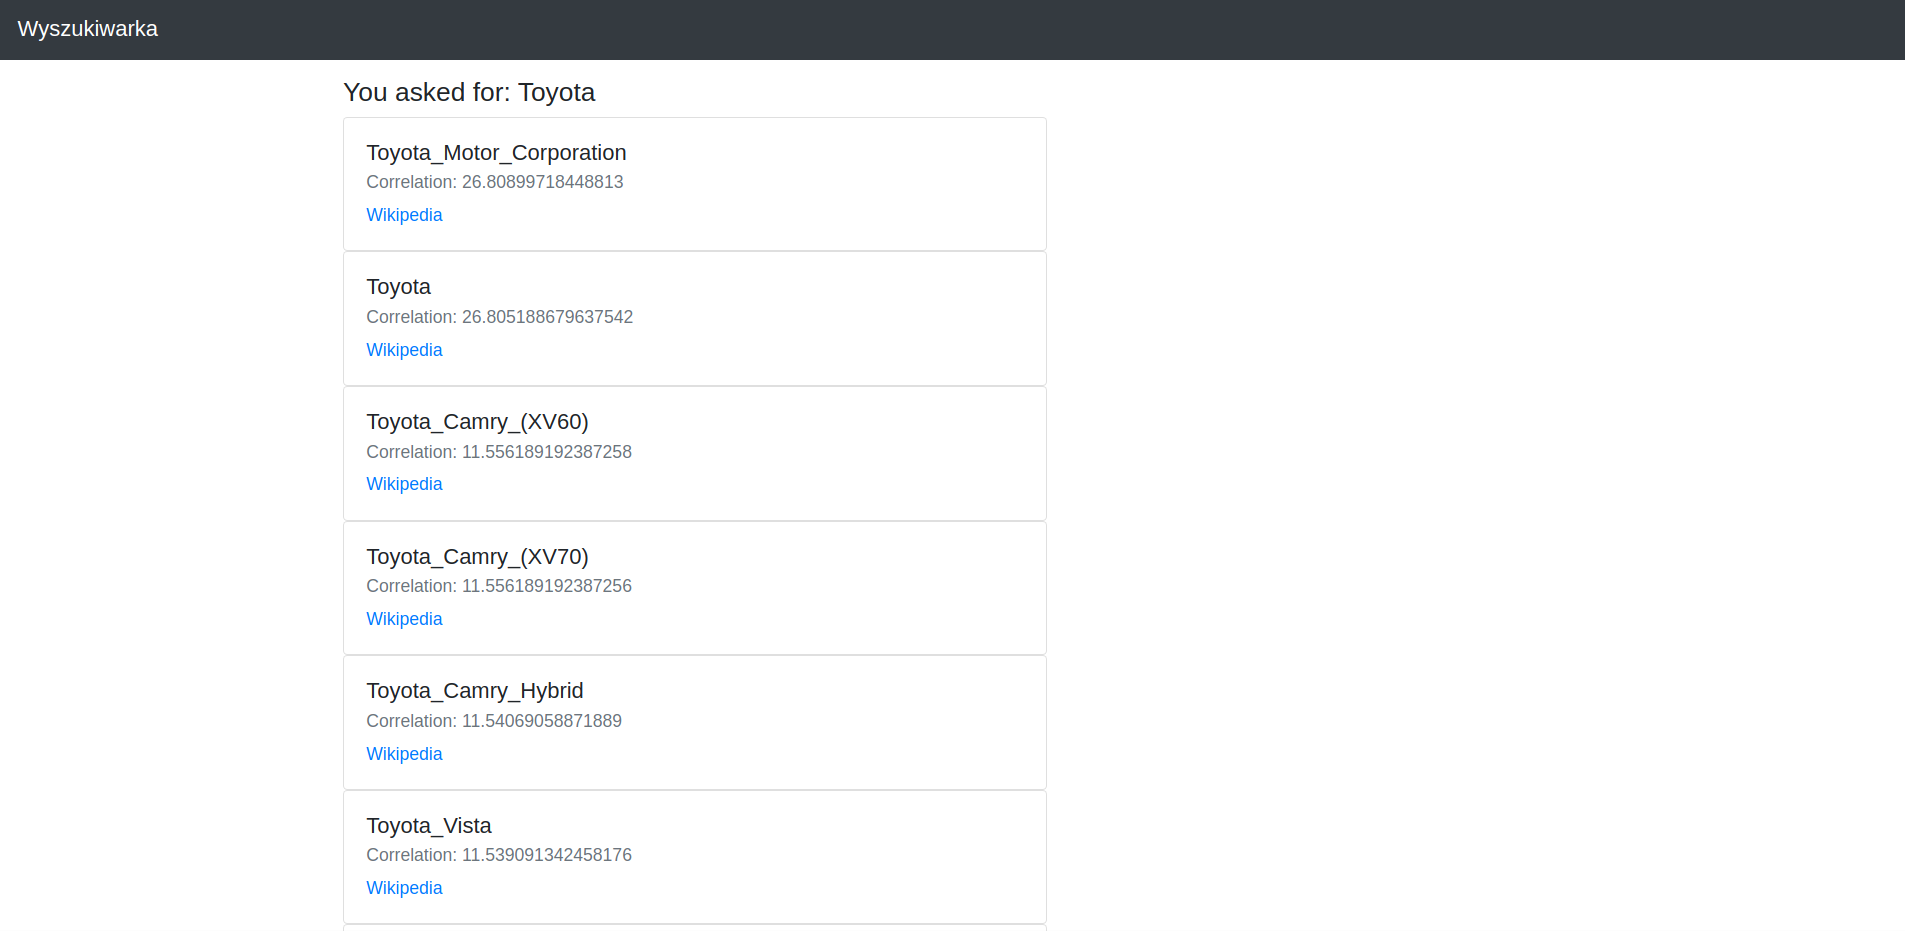
\includegraphics[height=10cm]{lab6/img/front_result1_k80.png}}
            \subfloat[$k=100$]{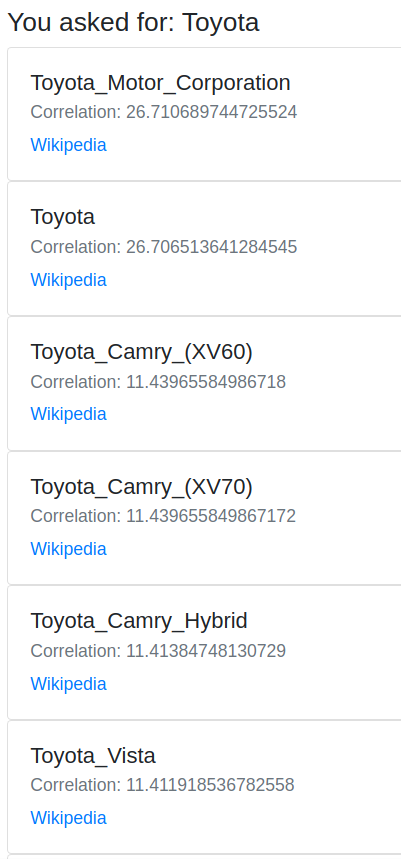
\includegraphics[height=10cm]{lab6/img/front_result1_k100.png}}
            \subfloat[$k=300$]{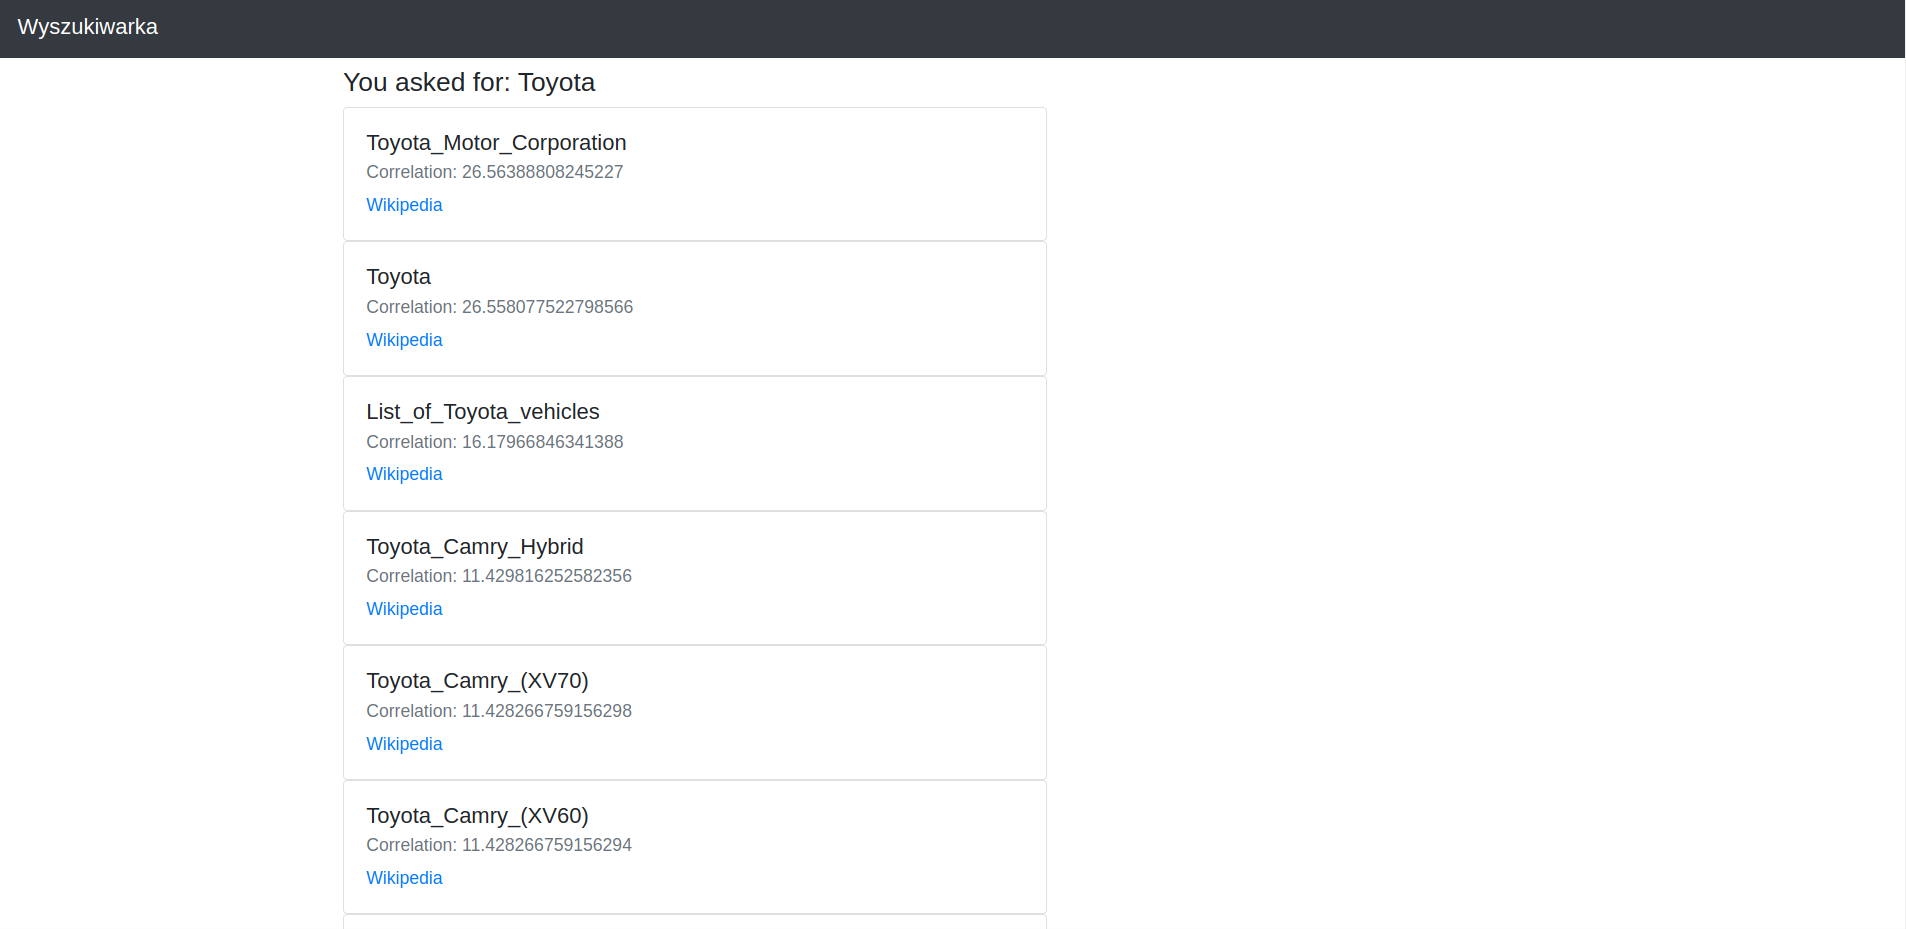
\includegraphics[height=10cm]{lab6/img/front_result1_idf_svd.png}}
            \caption{Zapytanie testowe: "Toyota"}
        \end{figure}
        \begin{figure}[h!]
            \centering
            \subfloat[$k=20$]{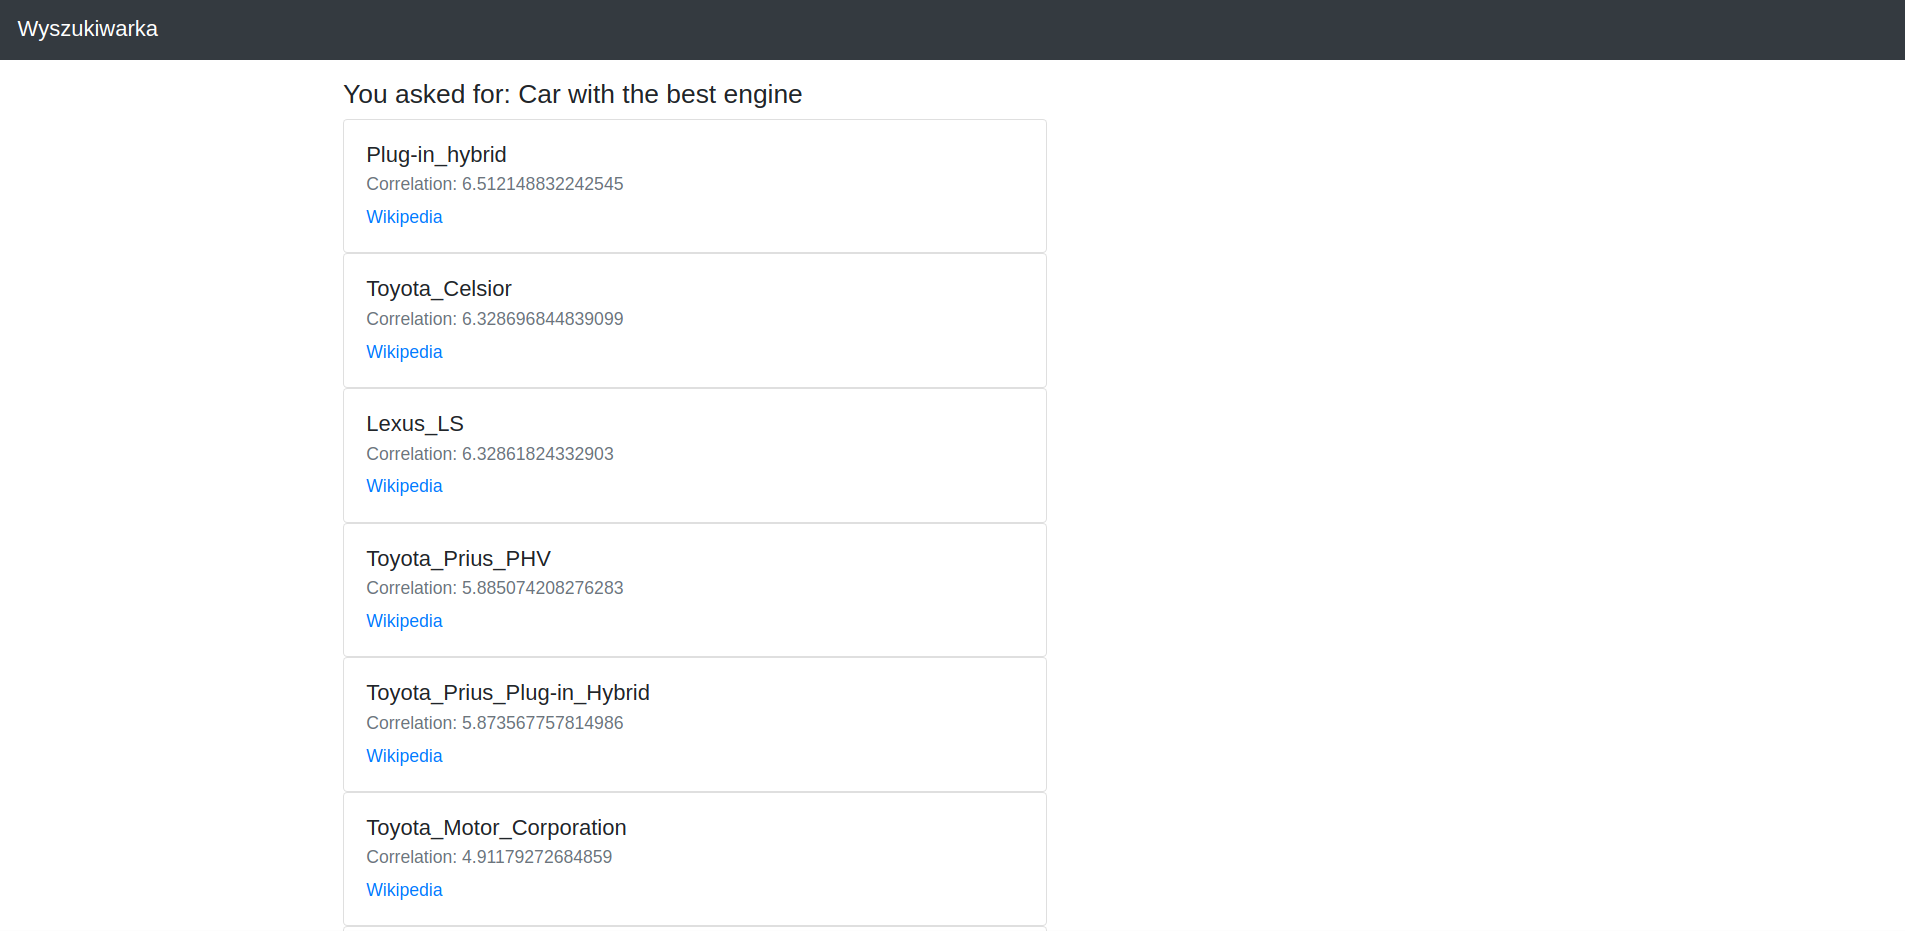
\includegraphics[height=10cm]{lab6/img/front_result2_k20.png}}
            \subfloat[$k=40$]{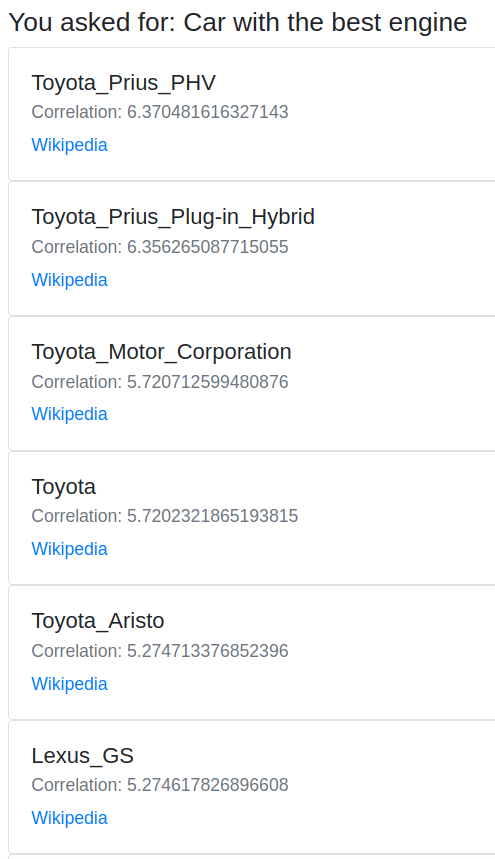
\includegraphics[height=10cm]{lab6/img/front_result2_k40.png}}
            \subfloat[$k=60$]{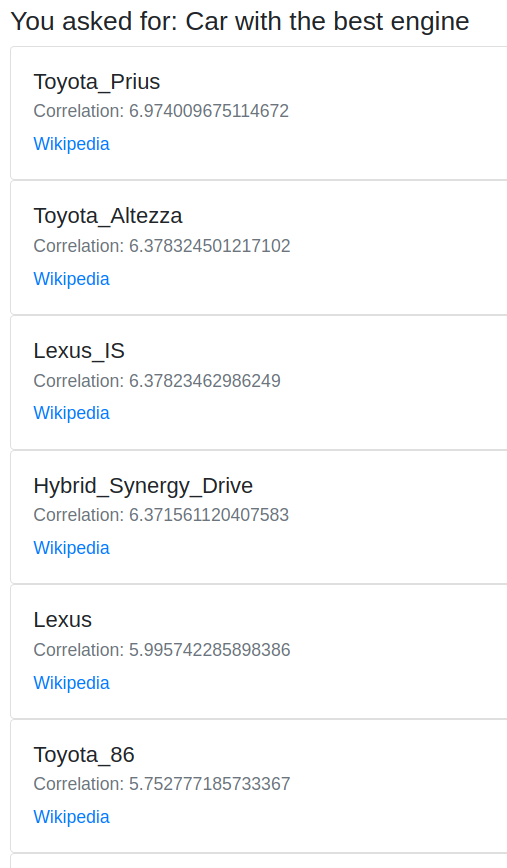
\includegraphics[height=10cm]{lab6/img/front_result2_k60.png}}\\
            \subfloat[$k=80$]{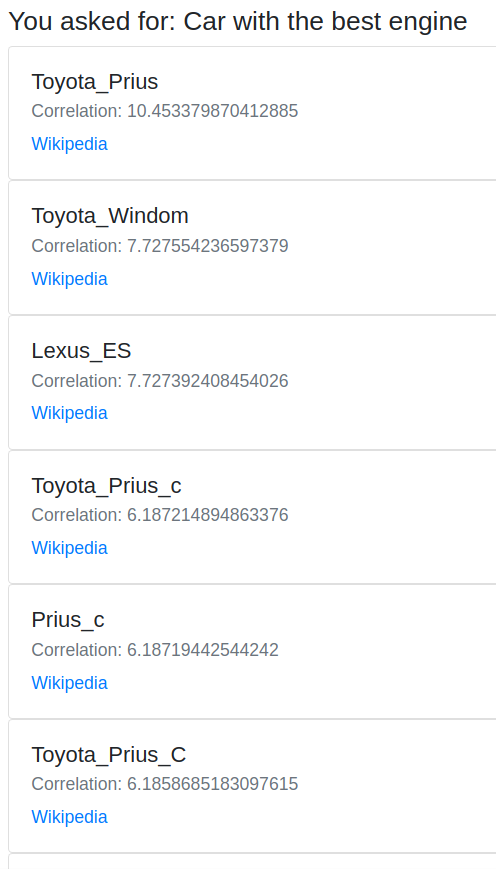
\includegraphics[height=10cm]{lab6/img/front_result2_k80.png}}
            \subfloat[$k=100$]{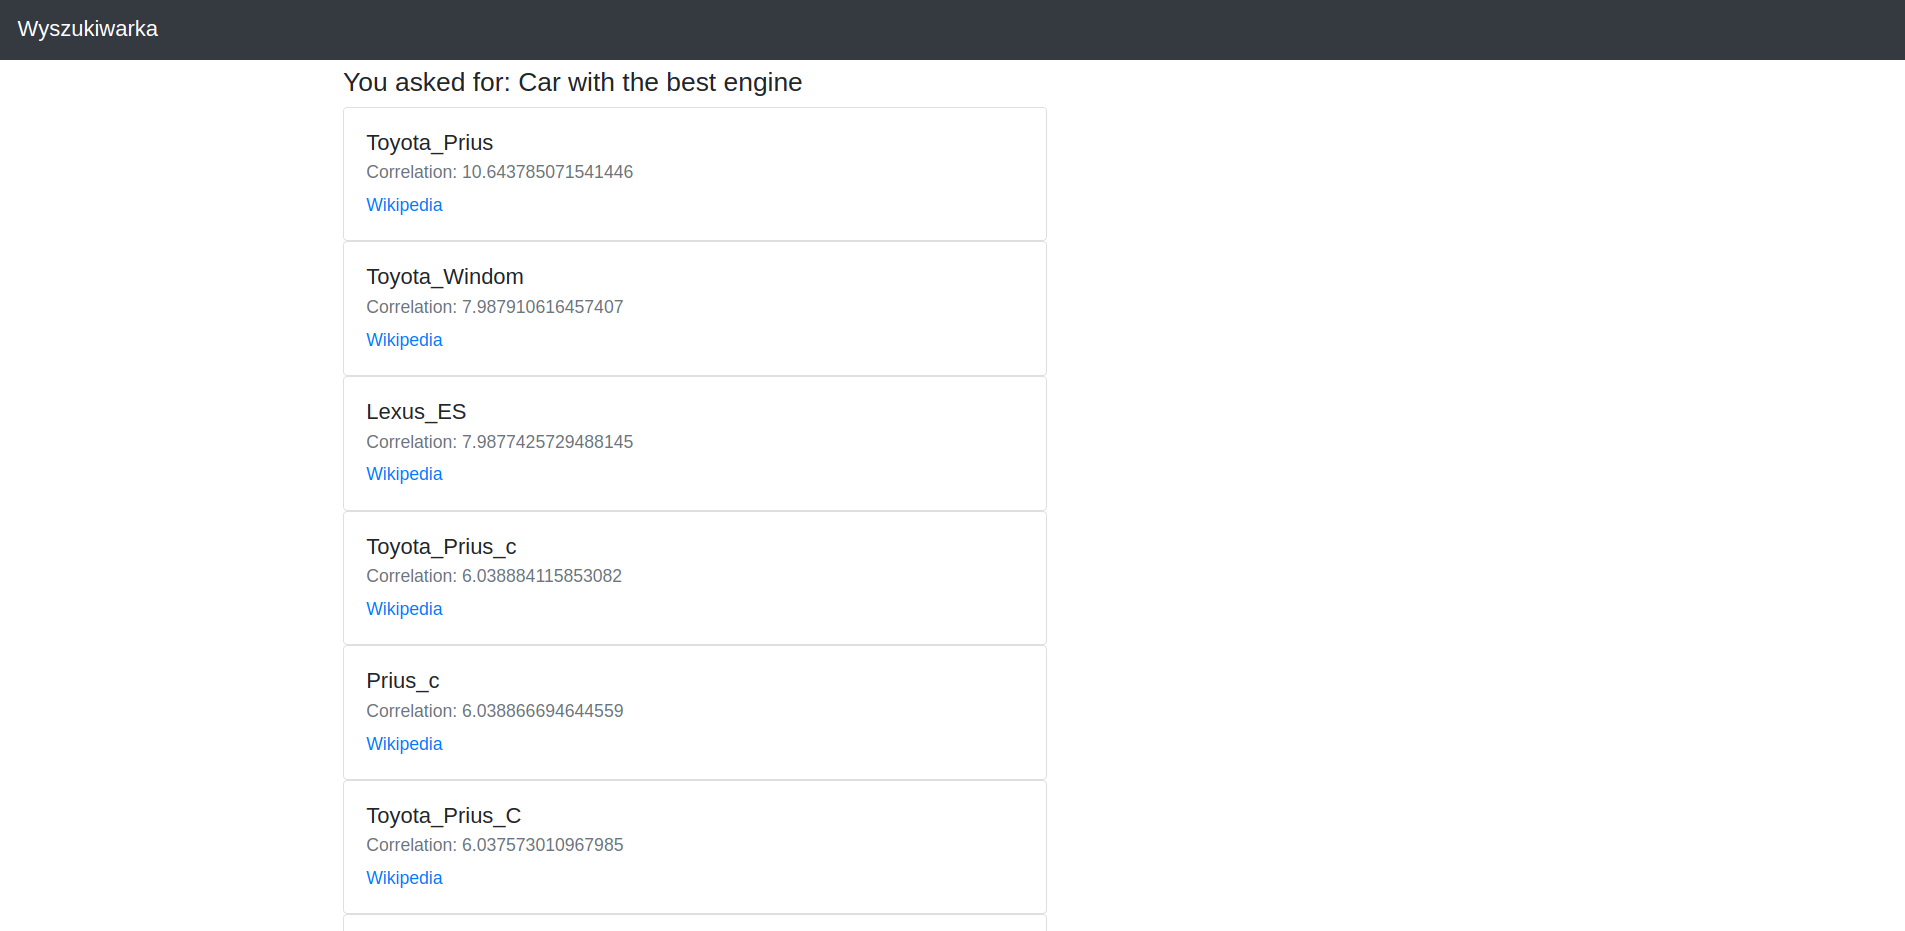
\includegraphics[height=10cm]{lab6/img/front_result2_k100.png}}
            \subfloat[$k=300$]{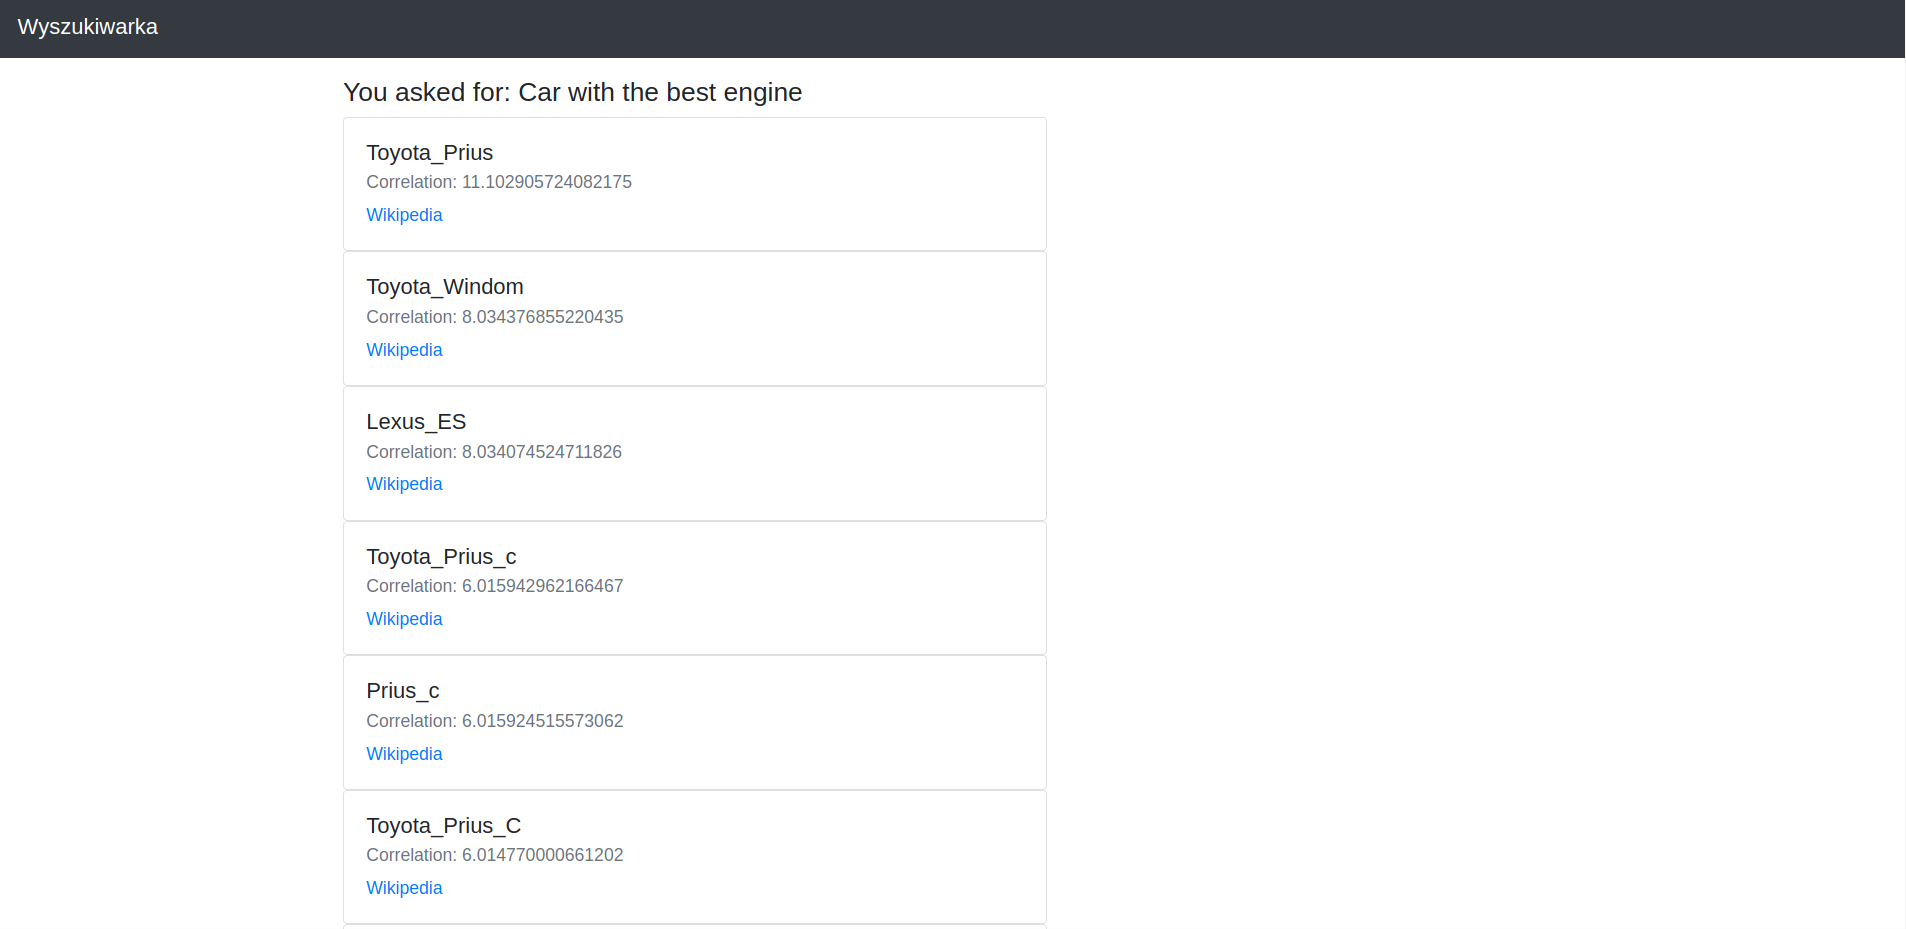
\includegraphics[height=10cm]{lab6/img/front_result2_idf_svd.png}}
            \caption{Zapytanie testowe: "Car with the best engine"}
        \end{figure}
        \begin{figure}[h!]
            \centering
            \subfloat[$k=20$]{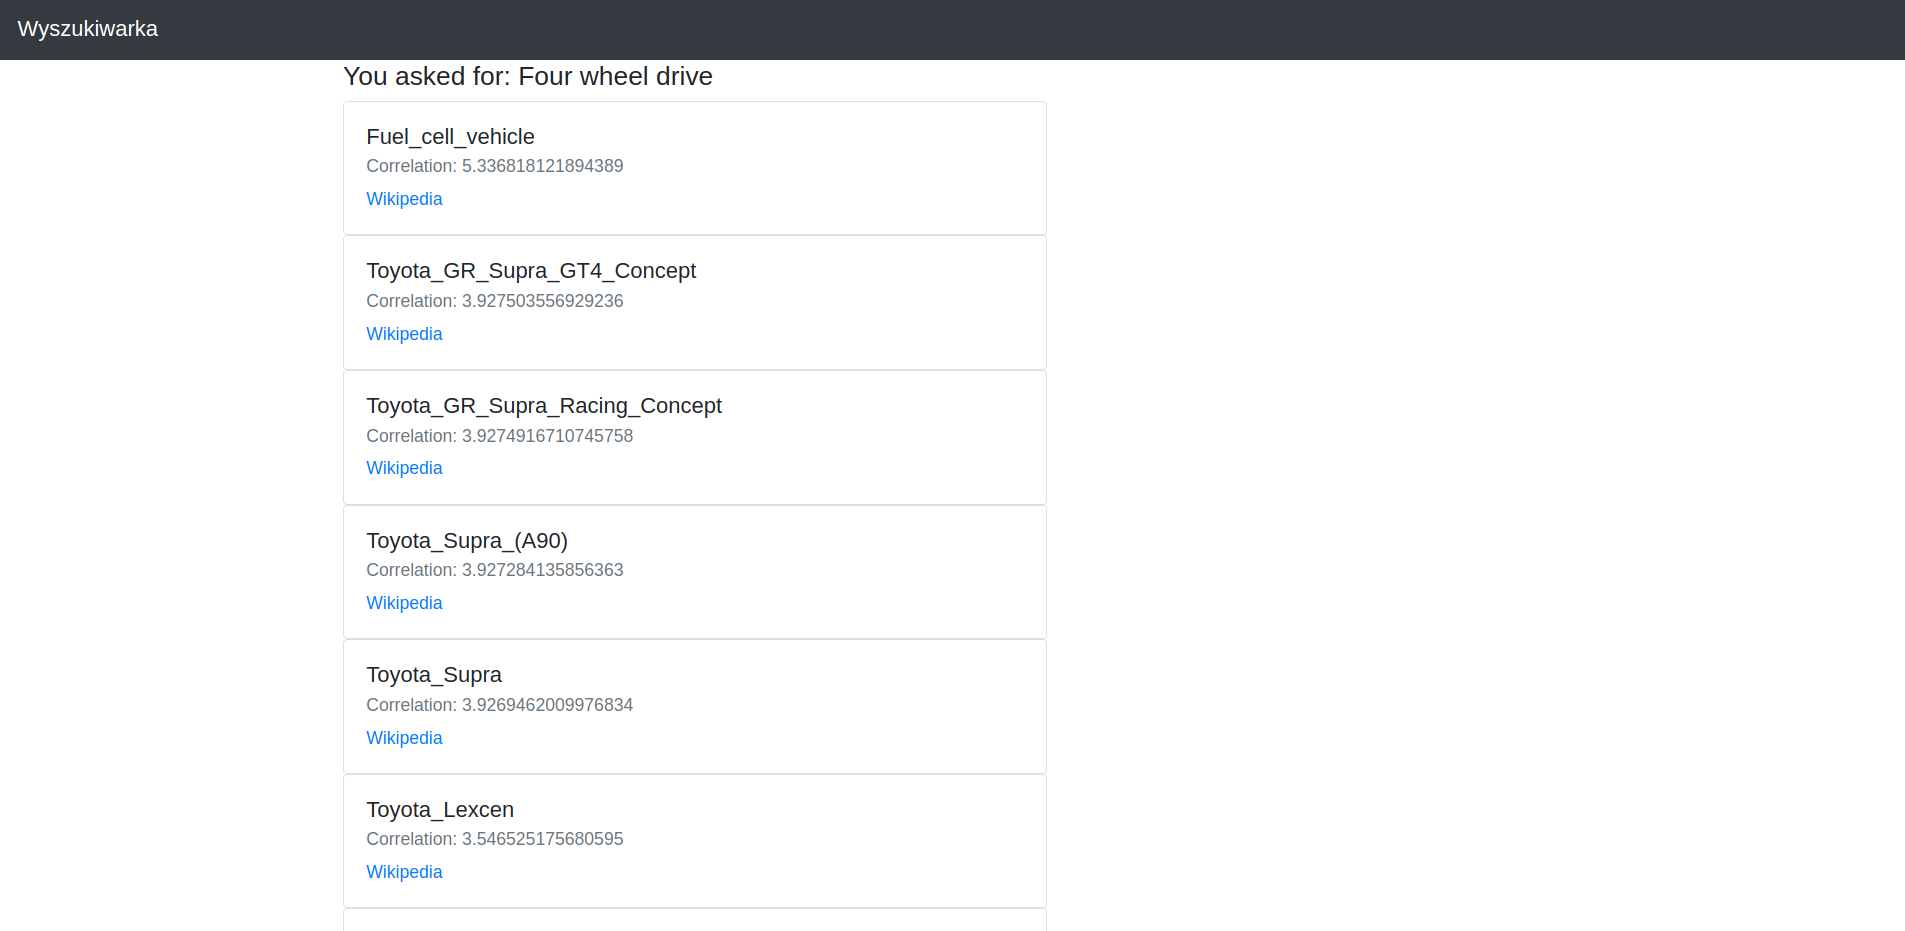
\includegraphics[height=10cm]{lab6/img/front_result3_k20.png}}
            \subfloat[$k=40$]{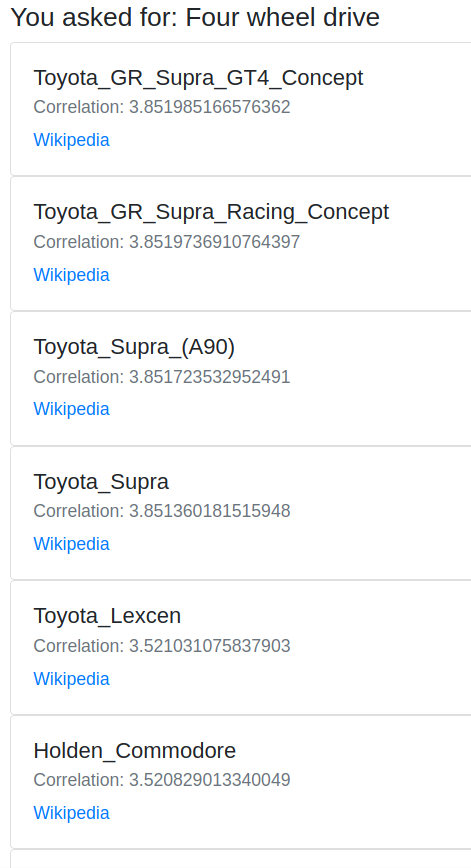
\includegraphics[height=10cm]{lab6/img/front_result3_k40.png}}
            \subfloat[$k=60$]{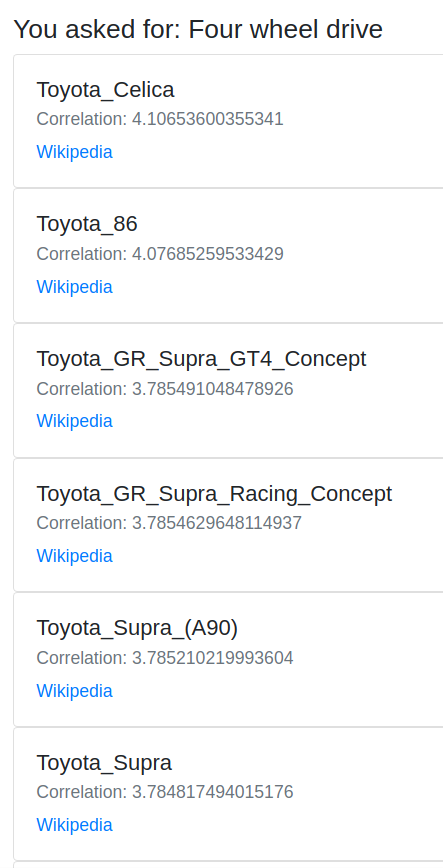
\includegraphics[height=10cm]{lab6/img/front_result3_k60.png}}\\
            \subfloat[$k=80$]{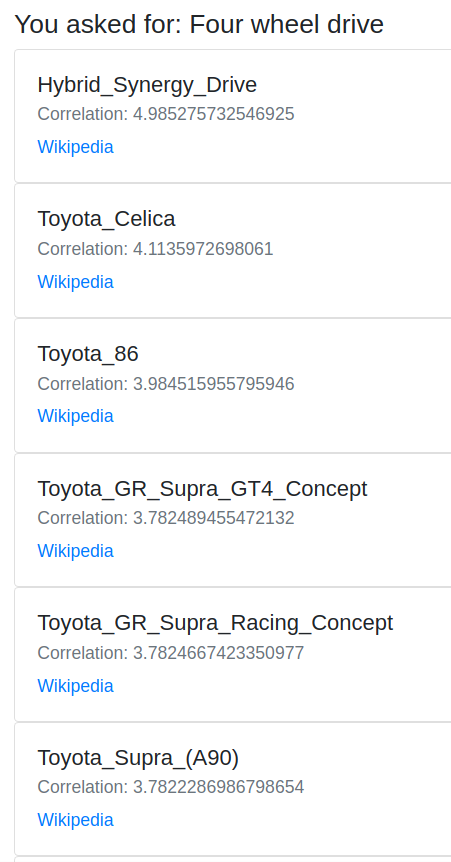
\includegraphics[height=10cm]{lab6/img/front_result3_k80.png}}
            \subfloat[$k=100$]{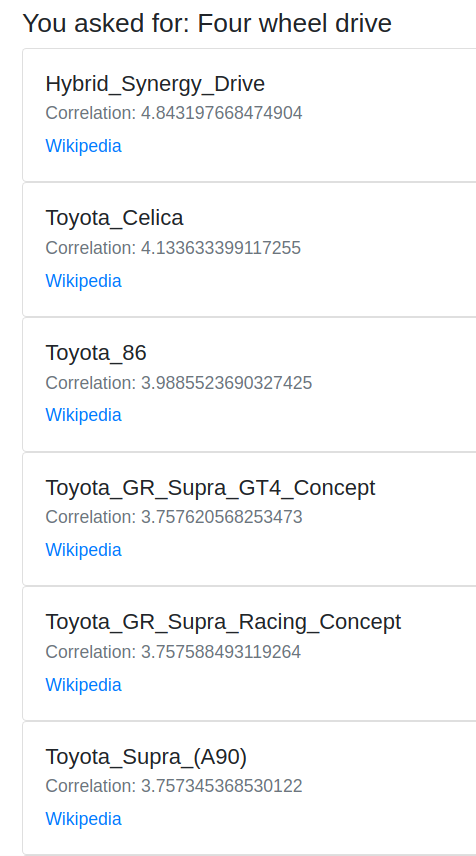
\includegraphics[height=10cm]{lab6/img/front_result3_k100.png}}
            \subfloat[$k=300$]{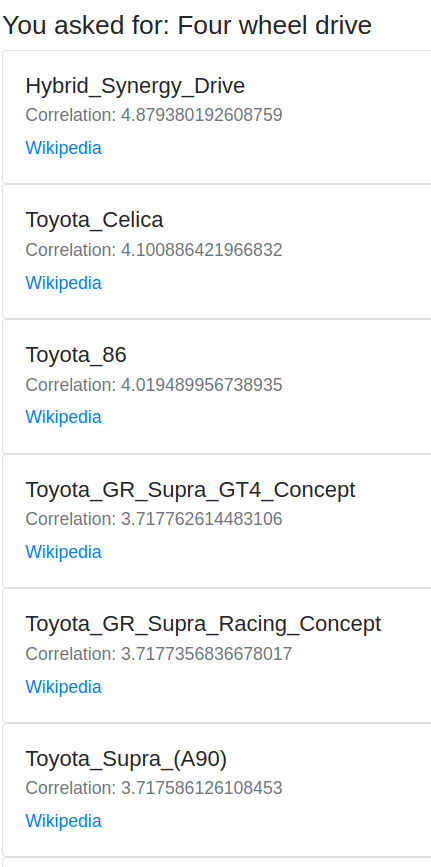
\includegraphics[height=10cm]{lab6/img/front_result3_idf_svd.png}}
            \caption{Zapytanie testowe: "Four wheel drive"}
        \end{figure}
        \newpage

        \subsection{Badanie wpływu transformacji IDF}
            Wykonałem też zapytania testowe mające wykazać wpływ transfomacji IDF na wyniki wyszukiwania.
            \begin{figure}[h!]
            \centering
            \subfloat[Bez IDF]{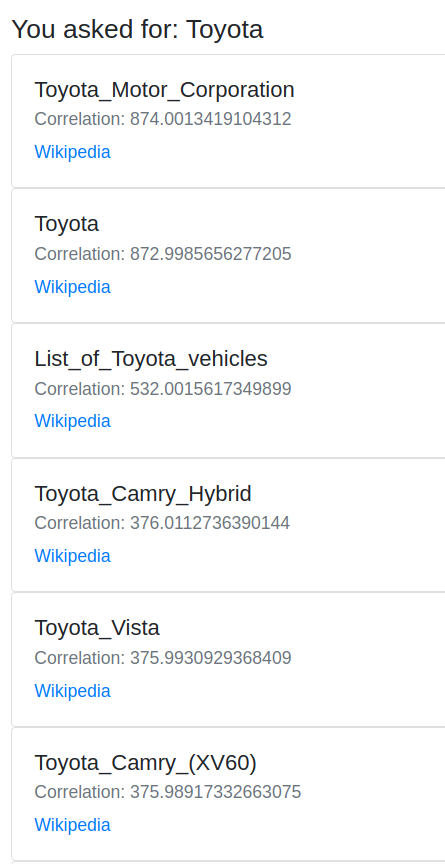
\includegraphics[height=10cm]{lab6/img/front_result1_svd.png}}
            \subfloat[Z IDF]{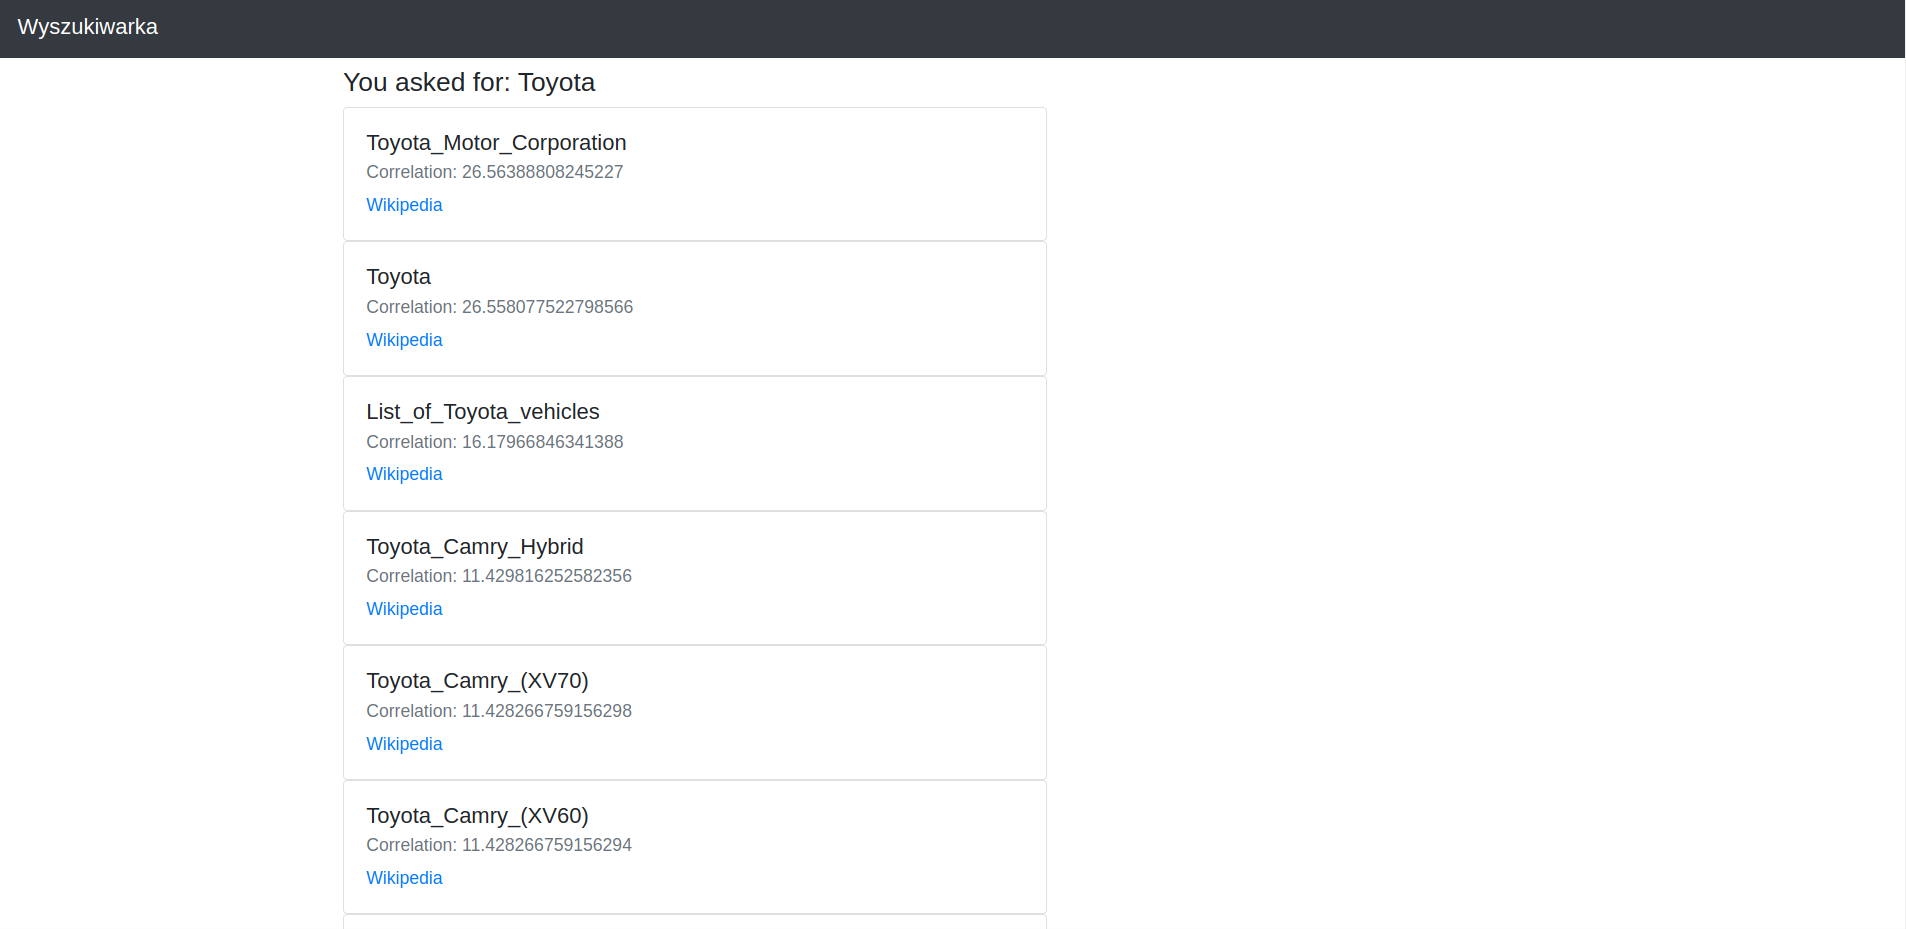
\includegraphics[height=10cm]{lab6/img/front_result1_idf_svd.png}}
            \subfloat[Bez IDF]{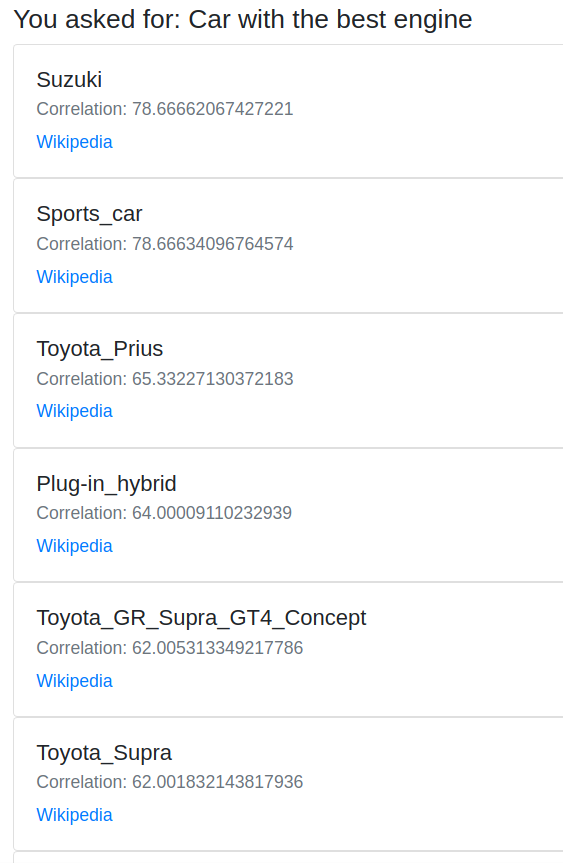
\includegraphics[height=10cm]{lab6/img/front_result2_svd.png}}\\
            \subfloat[Z IDF]{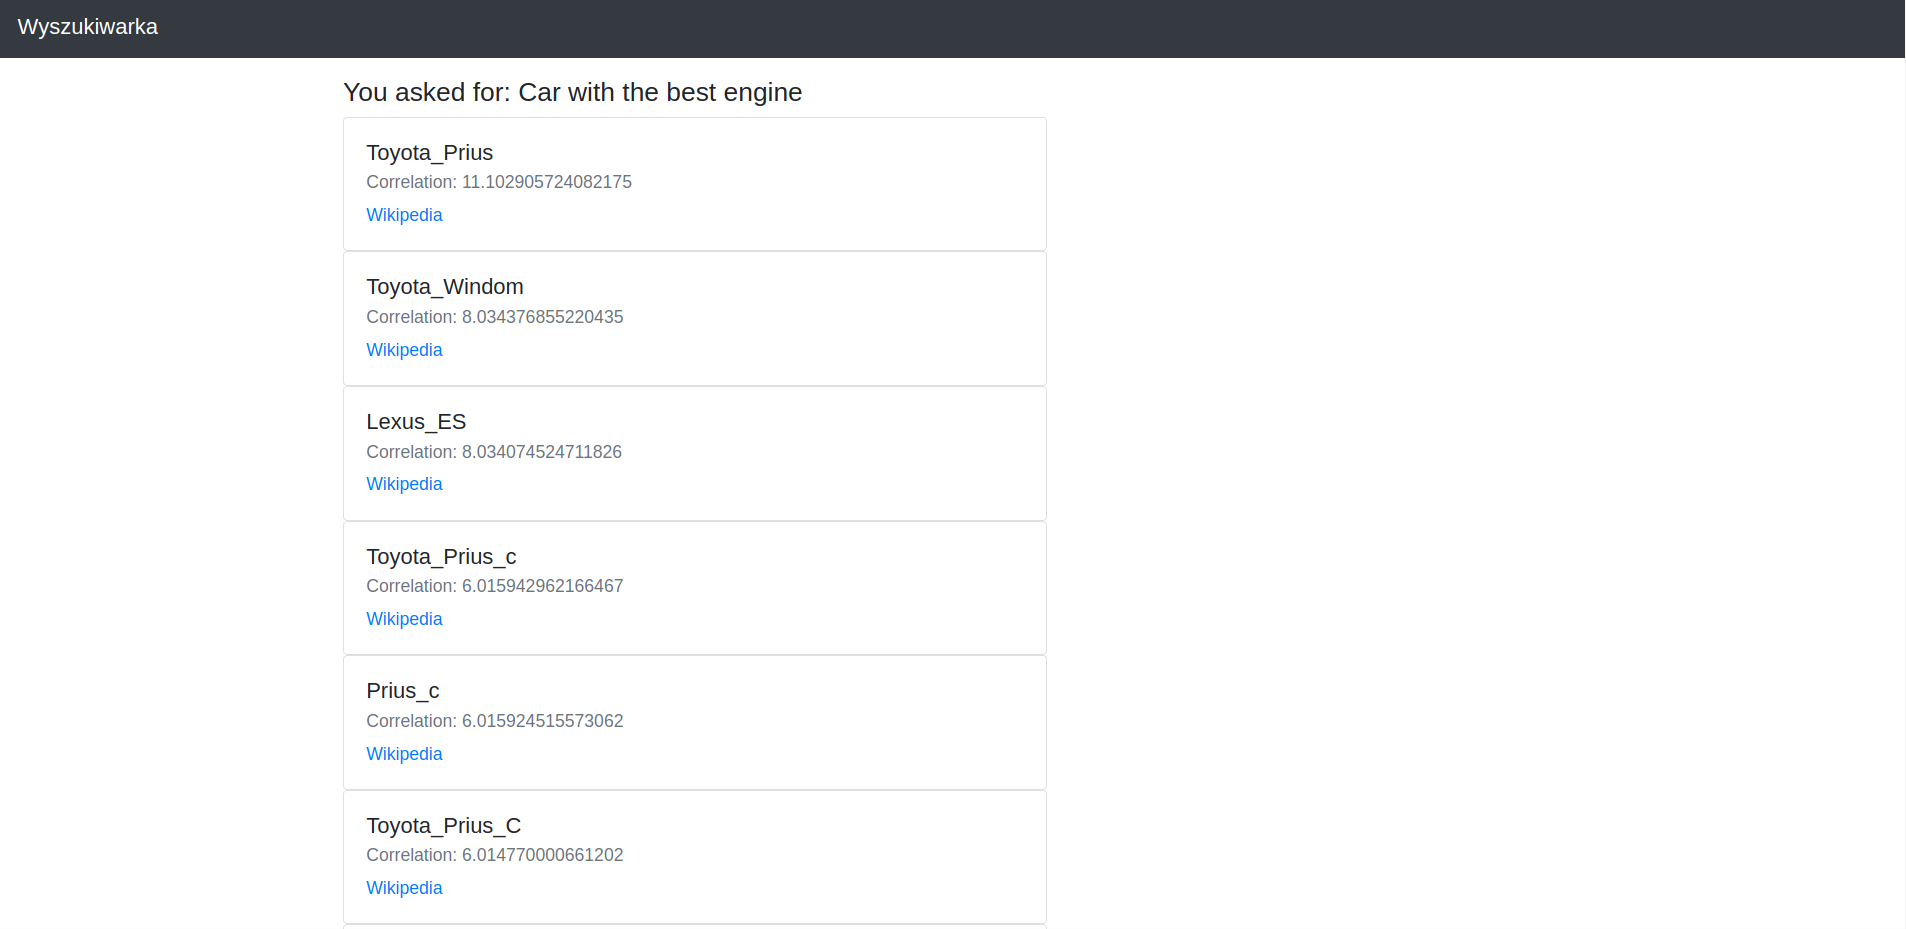
\includegraphics[height=10cm]{lab6/img/front_result2_idf_svd.png}}
            \subfloat[Bez IDF]{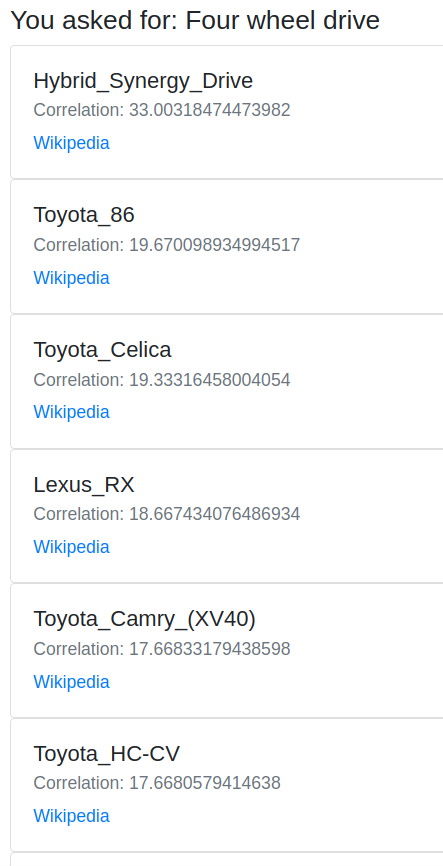
\includegraphics[height=10cm]{lab6/img/front_result3_svd.png}}
            \subfloat[Z IDF]{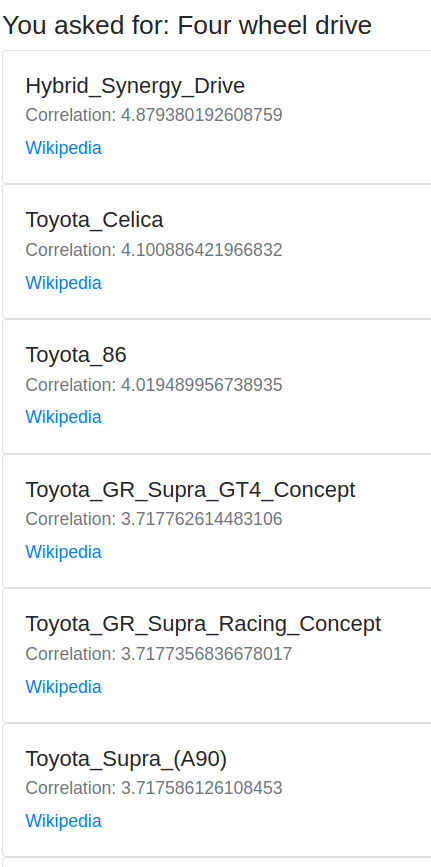
\includegraphics[height=10cm]{lab6/img/front_result3_idf_svd.png}}\\
            \subfloat[Bez IDF]{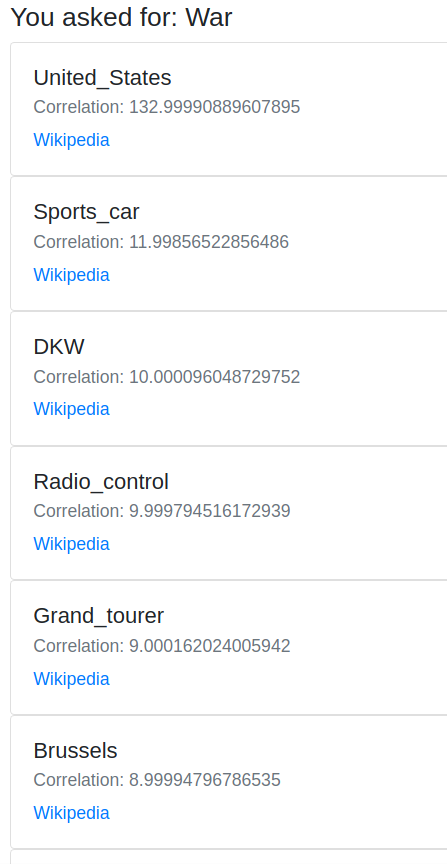
\includegraphics[height=10cm]{lab6/img/front_result4_svd.png}}
            \subfloat[Z IDF]{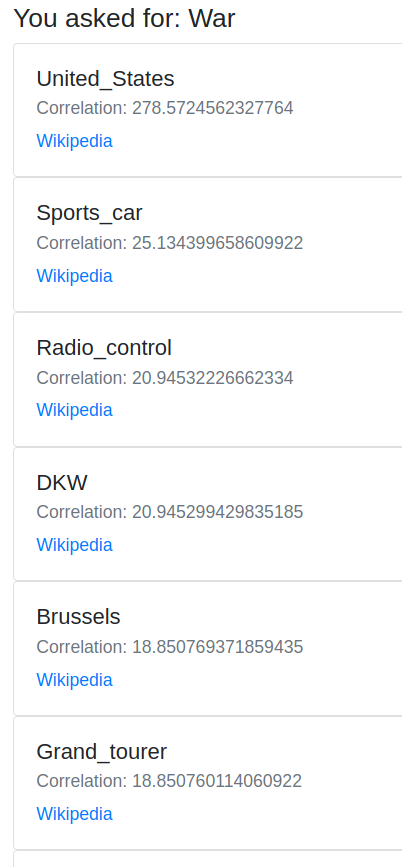
\includegraphics[height=10cm]{lab6/img/front_result4_idf_svd.png}}
            \caption{Zmiana wyników wyszukiwania po przeprowadzeniu transformacji IDF.}
        \end{figure}

            

\end{document}